% 5. Method 
\section{Method}

\subsection{System Overview}

The simulation is structured as a pipeline that executes once per physics
timestep.  At the start of each step the \texttt{SimulationManager} gathers
per-agent navigation data from Unity's NavMesh on the main thread---the only
point at which the CPU reads agent state---and packages it into a compact
struct array.  That array is uploaded to the GPU in a single
\texttt{ComputeBuffer.SetData} call, after which all physics computation runs
entirely inside the compute shader.  Seven GPU kernels execute in sequence:
position prediction, spatial hashing, density-based LOD assignment, one or
more Jacobi constraint passes, and a finalisation step that derives velocity
and commits the new position.  Results are asynchronously read back to the
main thread one to two frames later via Unity's \texttt{AsyncGPUReadback} API,
where they update \texttt{Transform} components and synchronise the NavMesh
agent positions.  No per-agent CPU computation occurs between the upload and
the readback.

The system exposes six interchangeable solver backends---\textit{Force},
\textit{ForceJobs}, \textit{PBD}, \textit{PBDJobs}, \textit{PBDCLODJobs}, and
\textit{PBDCompute}---selectable at runtime without restarting the simulation,
together with an additional culling-aware variant
(\textit{PBDCLODCullingJobs}).  This design makes it straightforward to
compare algorithmic choices and parallelism strategies against a common agent
population and scene configuration. 

%       Predict -> Clear -> Hash -> AssignLOD -> (Solve -> Apply) x N -> Finalize
\begin{figure}[h]
    \centering
    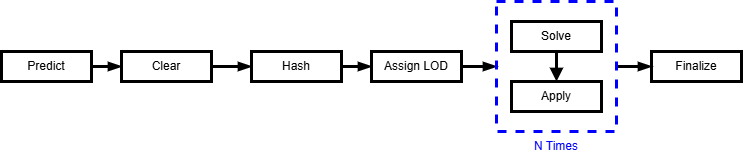
\includegraphics[width=0.7\textwidth]{pipelineDiagram.png}
    \caption{Solver pipeline diagram.  The main thread uploads agent data to the GPU, which executes the entire physics loop across multiple kernels.  Results are asynchronously read back to the CPU for Transform and NavMesh updates.}
    \label{fig:Solve_Pipeline}
\end{figure}


\subsection{Crowd Representation}

Each simulated pedestrian is represented by an \texttt{AgentBase} object on
the CPU side that stores world-space position, velocity, preferred speed,
radius, mass, and a reference to the Unity NavMeshAgent that provides
pathfinding.  For the GPU-accelerated solver this data is transcribed into a
tightly packed 64-byte \texttt{AgentGPU} struct whose layout is shared
verbatim between C\# and HLSL:

\begin{verbatim}
struct AgentGPU {
    float3 position;          // committed world position
    float  ksi;               // velocity blend factor [0,1]
    float3 predictedPosition; // working copy during solve
    float  radius;
    float3 velocity;
    float  mass;
    float3 preferredVelocity; // goal velocity from NavMesh
    int    lodLevel;          // 0=HIGH  1=MED  2=LOW
};
\end{verbatim}

The four \texttt{float3}--\texttt{float} pairs each occupy exactly 16 bytes,
satisfying the alignment requirements of both Metal and DirectX~12 without
padding.  The \texttt{lodLevel} field is written exclusively by the GPU on
every frame and is never uploaded from the CPU.

Navigation targets are computed on the main thread using Unity's NavMesh
steering API and supplied to each agent as a \texttt{preferredVelocity}
three-vector.  The preferred velocity encodes both direction and the agent's
desired walking speed, so the GPU solver requires no knowledge of goal
geometry or waypoint topology.

\subsection{CLOD Framework}

\subsubsection{Density Heatmap LOD (\textit{PBDCompute})}
\label{sec:clod_density}

The primary contribution of this work is a \emph{density-driven} continuous
level-of-detail system in which physics fidelity is allocated in proportion to
local crowd density rather than distance from the camera or player.  The
central observation is that collision resolution is only computationally
expensive when many agents are in proximity; a lone agent far from any crowd
requires almost no constraint work, whereas a dense cluster---regardless of
its screen-space size---demands full solver fidelity.

The density field is computed as a by-product of the spatial hashing step with
no additional memory or compute cost.  After \texttt{KernelHashAgents}, the
atomic counter array \texttt{\_HashGridCount[h]} holds exactly the number of
agents assigned to bucket $h$.  This constitutes the heatmap: each cell's
count is its density.  \texttt{KernelAssignLOD} then reads each agent's own
cell count and maps it to one of three tiers using two configurable integer
thresholds, $D_{\mathrm{high}}$ and $D_{\mathrm{med}}$ (defaults 12 and 4
respectively):

\begin{equation}
    \mathrm{LOD}(i) =
    \begin{cases}
        \text{\textsc{High}} & \text{if } \rho(i) > D_{\mathrm{high}} \\
        \text{\textsc{Med}}  & \text{if } \rho(i) > D_{\mathrm{med}}  \\
        \text{\textsc{Low}}  & \text{otherwise}
    \end{cases}
\end{equation}

where $\rho(i)$ is the agent count of the cell containing agent $i$.  The
assignment is performed every frame without hysteresis or temporal smoothing:
because density changes slowly relative to the physics timestep, flickering
between tiers is rare in practice, and the absence of hysteresis keeps the
kernel stateless and branchless.

The three tiers differ in the spatial extent of their neighbour search and the
number of collision contacts resolved per Jacobi pass:

\begin{center}
\begin{tabular}{lccc}
\hline
\textbf{Tier} & \textbf{Density condition} & \textbf{Search region} & \textbf{Max contacts} \\
\hline
High & $\rho > 12$ & $3\times3$ cell neighbourhood & 12 \\
Med  & $4 < \rho \leq 12$ & Centre cell only & 4 \\
Low  & $\rho \leq 4$ & Centre cell only & 1 \\
\hline
\end{tabular}
\end{center}

Every agent is solved on every frame regardless of tier; there is no
frame-offset skipping.  This eliminates the temporal artefacts that arise when
distant or sparse agents resolve constraints only every $k$-th frame.

\subsubsection{Camera-Distance CLOD (\textit{PBDCLODJobs})}
\label{sec:clod_camera}

An earlier solver variant implements a camera-distance approach in which each
agent's LOD tier is determined by its Euclidean distance from a designated
focus point (typically the player or main camera).  Two configurable radii,
$r_{\mathrm{high}}$ and $r_{\mathrm{med}}$, partition the scene into
concentric zones.  A 10\% hysteresis band prevents agents from oscillating
between tiers at zone boundaries.  An additional density-aware promotion rule
inspects the previous frame's correction count: agents that resolved five or
more contacts are promoted one tier regardless of distance, ensuring that
pockets of high density are handled with appropriate fidelity even when they
fall outside the high-LOD radius.

Low-tier agents in this variant skip constraint resolution on three out of
every four frames (gated by \texttt{frameCount \% 4}), saving constraint work
at the cost of temporal jitter for distant agents.  The spatial hash is
built once per frame rather than once per iteration as a deliberate
performance trade-off; because predicted positions change by only small amounts
between Jacobi passes, a single hash is sufficient for neighbour lookup without
meaningful quality loss.

\subsubsection{Frustum-Culling CLOD (\textit{PBDCLODCullingJobs})}
\label{sec:clod_culling}

The culling solver extends \textit{PBDCLODJobs} with a fourth LOD tier,
\textsc{Culled}, for agents that lie outside the protagonist camera's view
frustum.  Culled agents have their \texttt{Renderer} and \texttt{Animator}
components disabled, eliminating all GPU draw calls and CPU skinning cost.
Their \texttt{Transform} position is still written every frame so that NavMesh
pathfinding remains accurate and agents re-enter the visible scene smoothly.
Culled agents are also inserted into the spatial hash so they continue to
function as collision obstacles for neighbours near the FOV boundary.

The frustum test uses all six camera planes extracted from the
\texttt{GeometryUtility.\allowbreak CalculateFrustumPlanes}  on the main thread (the
Camera API is unavailable inside Burst-compiled jobs).  Each plane's
distance is
expanded outward by a configurable margin (default 1.5 world units) so that
agents remain visible briefly after crossing the true boundary, hiding the
one-frame readback lag.  Renderer and Animator toggling is gated on a
per-agent \texttt{bool[]} change-detection array to avoid the hidden overhead
of redundant Unity component property writes.

\subsection{PBD Solver}
\label{sec:pbd_solver}

The position-based dynamics formulation follows Weiss, et al. 2019
\cite{weiss2019}.  Each timestep consists of three phases: prediction,
constraint projection, and finalisation.

\paragraph{Prediction.}
Each agent's velocity is blended toward its preferred velocity:
\begin{equation}
    \mathbf{v}_i \leftarrow (1 - \xi_i)\,\mathbf{v}_i + \xi_i\,\mathbf{v}^{\mathrm{pref}}_i
\end{equation}
where $\xi_i \in [0,1]$ controls the response rate.  The predicted position
is then computed by explicit Euler integration, pinned to the agent's current
$y$-coordinate to prevent vertical drift:
\begin{equation}
    \tilde{\mathbf{x}}_i \leftarrow \mathbf{x}_i + \mathbf{v}_i\,\Delta t, \qquad
    \tilde{x}_{i,y} \leftarrow x_{i,y}.
\end{equation}

\paragraph{Short-Range Collision Constraint.}
For each overlapping agent pair $(i,j)$ with combined radius
$r_{ij} = r_i + r_j$ and contact normal
$\mathbf{n} = (\tilde{\mathbf{x}}_i - \tilde{\mathbf{x}}_j)/d_{ij}$
where $d_{ij} = \|\tilde{\mathbf{x}}_i - \tilde{\mathbf{x}}_j\|$,
the Jacobi correction applied to agent $i$ is:
\begin{equation}
    \Delta\mathbf{x}_i = -\frac{w_i}{w_i + w_j}\,k_{\mathrm{sr}}\,
    (d_{ij} - r_{ij})\,\mathbf{n}
\end{equation}
where $w_i = 1/m_i$ are inverse masses and $k_{\mathrm{sr}} \in [0,1]$ is a
stiffness coefficient.  A tangential friction term is appended by decomposing
the relative displacement $\Delta\mathbf{r} = (\tilde{\mathbf{x}}_i + \Delta\mathbf{x}_i -
\mathbf{x}_i) - (\tilde{\mathbf{x}}_j - \Delta\mathbf{x}_j - \mathbf{x}_j)$
into normal and tangential components and applying a Coulomb-like clamp:
\begin{equation}
    \Delta\mathbf{x}^{\mathrm{tan}}_i =
    w_i \min\!\left(\frac{\mu_k\,d_{ij}}{|\Delta\mathbf{r}^{\mathrm{tan}}|},\;1\right)
    \Delta\mathbf{r}^{\mathrm{tan}}
    \quad \text{when } |\Delta\mathbf{r}^{\mathrm{tan}}| \geq \mu_s\,d_{ij}
\end{equation}
where $\mu_s$ and $\mu_k$ are the static and kinetic friction coefficients.

\paragraph{Long-Range Collision Constraint.}
For \textsc{High}-tier agents, a predictive avoidance constraint is applied
following the time-of-impact formulation of \cite{weiss2019}.  Given relative
position $\mathbf{x}_{ij} = \mathbf{x}_i - \mathbf{x}_j$ and relative
velocity $\mathbf{v}_{ij}$, the time to collision $t$ is the smaller positive
root of:
\begin{equation}
    |\mathbf{v}_{ij}|^2\,t^2 - 2(\mathbf{x}_{ij}\cdot\mathbf{v}_{ij})\,t
    + |\mathbf{x}_{ij}|^2 - r_{ij}^2 = 0.
\end{equation}
If $t \in (0,\,t_0]$ where $t_0$ is the configurable look-ahead window, a
correction proportional to $k_{\mathrm{lr}}\,\Delta t / t$ is applied in the
direction of the predicted contact normal, causing agents to steer apart before
the collision occurs.

\paragraph{Jacobi Iteration.}
Corrections are accumulated into a separate buffer during each constraint pass
and applied at its end.  This Jacobi scheme is unconditionally parallelisable:
every thread reads from the unmodified \texttt{\_Agents} buffer and writes
only to \texttt{\_Corrections}, eliminating write--write hazards without
double-buffering the full agent array.  The position update is:
\begin{equation}
    \tilde{\mathbf{x}}_i \leftarrow \tilde{\mathbf{x}}_i
    + \alpha \cdot \frac{\displaystyle\sum_j \Delta\mathbf{x}_{ij}}{N_{\mathrm{contacts}}}
\end{equation}
where $\alpha$ is a configurable smoothing coefficient.

\paragraph{Finalisation.}
Velocity is derived from the constrained displacement:
\begin{equation}
    \mathbf{v}_i \leftarrow (\tilde{\mathbf{x}}_i - \mathbf{x}_i) / \Delta t,
    \qquad \mathbf{x}_i \leftarrow \tilde{\mathbf{x}}_i.
\end{equation}

\subsection{Compute Shader Implementation}

\paragraph{Memory layout.}
All agent data lives in a single \texttt{RWStructuredBuffer<AgentGPU>}
allocated once per simulation initialisation and reused across frames.  The
64-byte struct fits exactly four 16-byte SIMD registers, minimising bank
conflicts in global memory reads on both Nvidia and Apple GPU architectures.
Corrections stored in a separate \texttt{RWStructuredBuffer<CorrectionData>}
(16 bytes: \texttt{float3} plus \texttt{int}) to preserve the Jacobi
read/write separation without duplicating the larger agent struct.

\paragraph{Spatial hash and density map.}
The spatial hash is implemented as two flat integer arrays:
\texttt{\_HashGrid[HASH\_BUCKET\_COUNT $\times$ MAX\_PER\_BUCKET]} stores
agent indices and \texttt{\_HashGridCount[HASH\_BUCKET\_COUNT]} stores
per-bucket occupancy.  The bucket count is fixed at 8192 (a power of two) to
allow bitmask indexing: $h = (c_x \cdot p_1) \oplus (c_z \cdot p_2) \;\&\;
M$ where $p_1$, $p_2$ are large primes and $M = 8191$.  Overflow beyond
\texttt{MAX\_PER\_BUCKET} (16) agents per bucket is silently clamped; at
typical crowd densities with a cell size of 4 world units this condition is
rare.  Atomic insertion uses \texttt{InterlockedAdd}, which is natively
supported on all DX11 and Metal~2 targets.  The \texttt{\_HashGridCount}
array serves double duty: after \texttt{KernelHashAgents} it contains the
per-cell density values that \texttt{KernelAssignLOD} reads to determine each
agent's LOD tier.

\paragraph{Dispatch sizing.}
All kernels use a thread group size of 64, matching the recommended warp/wave
size for cross-platform GPU code.  The number of agent thread groups is
$\lceil N/64 \rceil$, computed once at initialisation.  The clear kernel uses
$\lceil (B \times M)/64 \rceil$ groups to cover both hash arrays, where $B$
is the bucket count and $M$ is the slots per bucket.  Storing these counts
avoids per-frame integer division.

\paragraph{CPU--GPU data flow.}
The only CPU-to-GPU transfer per frame is a single \texttt{SetData} call on
the agent buffer ($N \times 64$ bytes).  All intermediate data---hash grid,
corrections, updated positions---remains on the GPU across the constraint
iterations.  Results are retrieved via \texttt{AsyncGPUReadback}, which
schedules a DMA transfer that completes on the main thread without stalling
the render pipeline.  A version counter incremented on each \texttt{Init}
call ensures that callbacks from stale simulations (e.g.\ triggered by a
scene respawn between the dispatch and the readback) are silently discarded
rather than applied to the new agent list.

\paragraph{Kernel sequence.}
The seven kernels are dispatched in sequence by the C\# \texttt{Solve} method.
Unity's \texttt{\allowbreak ComputeShader.Dispatch} inserts an implicit UAV pipeline
barrier between calls, so no explicit memory fences are required:

\begin{enumerate}
    \item \texttt{KernelPredict} --- velocity blend and Euler integration (once per frame).
    \item \texttt{KernelClearHashGrid} --- zero density map and entry slots (once per frame).
    \item \texttt{KernelHashAgents} --- atomic insertion; populates the density heatmap (once per frame).
    \item \texttt{KernelAssignLOD} --- density threshold $\rightarrow$ \texttt{lodLevel} (once per frame).
    \item \texttt{KernelSolveConstraints} --- Jacobi solve with LOD-gated search ($N_{\mathrm{iter}}$ times).
    \item \texttt{KernelApplyCorrections} --- averaged delta into \texttt{predictedPosition} ($N_{\mathrm{iter}}$ times).
    \item \texttt{KernelFinalize} --- commit velocity and position (once per frame).
\end{enumerate}

\subsection{Other Solver Variants}

\subsubsection{Force Solver (\textit{Force})}

The baseline solver implements the Social Force Model of
Helbing, et al. 2001 \cite{helbing1995}.  Each agent computes a
driving force toward its current goal and a set of repulsive avoidance forces
from nearby agents.  The avoidance force for a pair $(i,j)$ is derived from
the predicted time to collision $t$, yielding a repulsion that grows sharply
as collision becomes imminent.  Neighbour queries use a main-thread spatial
grid rebuilt each frame.  This solver is single-threaded and serves as a
correctness and performance baseline.

\subsubsection{Parallelised Force Solver (\textit{ForceJobs})}

This variant parallelises the Social Force computation across Unity's C\# Job
System with Burst compilation.  Agent data is packed into a
\texttt{NativeArray<ForceAgentData>}, a parallel hash-insertion job populates
a \texttt{NativeParallelMultiHashMap}, and a parallel force-calculation job
reads from it.  Wall repulsion forces generated by NavMesh obstacle geometry
are applied on the main thread after \texttt{handle.Complete()} because the
managed \texttt{Bounds} list is not accessible inside Burst-compiled code.

\subsubsection{Single-Threaded PBD Solver (\textit{PBD})}

This solver implements the PBD loop of Section~\ref{sec:pbd_solver} entirely
on the main CPU thread.  Neighbour queries use the pre-built main-thread
spatial grid.  The finalisation step includes a rebound-suppression heuristic:
outgoing speed is clamped to 115\% of the preferred speed, and the component
of velocity directed away from the goal is attenuated to prevent elastic
bounce artefacts after a penetration is resolved.

\subsubsection{Parallelised PBD Solver (\textit{PBDJobs})}

This solver distributes the predict, hash, constraint, apply, and update steps
across Burst-compiled \texttt{IJobParallelFor} jobs chained by
\texttt{JobHandle} dependencies.  The spatial hash is rebuilt inside the job
pipeline on every constraint iteration (unlike \textit{PBDCLODJobs} which
hashes once per frame), giving fresher neighbour data at the cost of
additional hashing overhead per iteration.  Transform writes are deferred to
an \texttt{IJobParallelForTransform} job that operates in parallel with the
final velocity derivation.

\subsubsection{Camera-Distance CLOD PBD Solver (\textit{PBDCLODJobs})}

This solver introduces the three-tier camera-distance LOD system described in
Section~\ref{sec:clod_camera} and is the most feature-complete of the CPU-side
solvers.  Four \texttt{NativeList<int>} arrays separate agents by tier; each
tier schedules its own constraint job with the appropriate search radius and
contact budget.  Adaptive LOD scaling automatically reduces tier radii when
the frame rate falls below a configurable target, providing load shedding under
GPU pressure without manual tuning.

\subsubsection{Frustum-Culling CLOD Solver (\textit{PBDCLODCullingJobs})}

This solver extends \textit{PBDCLODJobs} with the \textsc{Culled} tier
described in Section~\ref{sec:clod_culling}.  The frustum-plane computation
runs on the main thread before job scheduling and the six planes are passed to
the categorisation job as a \texttt{NativeArray<float4>}.  Rotation
interpolation is skipped for culled agents in the transform job, saving one
quaternion slerp per culled agent per frame with no visual consequence since
the renderer is disabled.